\documentclass{standalone}
\usepackage{tikz}
\usepackage{graphicx}

\usetikzlibrary{calc}
\usetikzlibrary{angles,quotes} % for pic
\usetikzlibrary{patterns,snakes}
\usetikzlibrary{arrows}
\usetikzlibrary{shapes.geometric, arrows}

\tikzstyle{startstop} = [rectangle, rounded corners, minimum width=3cm, minimum height=1cm,text centered, draw=black, fill=red!30]
\tikzstyle{process} = [rectangle, minimum width=3cm, minimum height=1cm, text centered, draw=black, fill=orange!30]
\tikzstyle{decision} = [diamond, minimum width=3cm, minimum height=1cm, text centered, draw=black, fill=green!30]
\tikzstyle{io} = [trapezium, trapezium left angle=70, trapezium right angle=110, minimum width=3cm, minimum height=1cm, text centered, draw=black, fill=blue!30]
\tikzstyle{arrow} = [thick,->,>=stealth]


\begin{document}
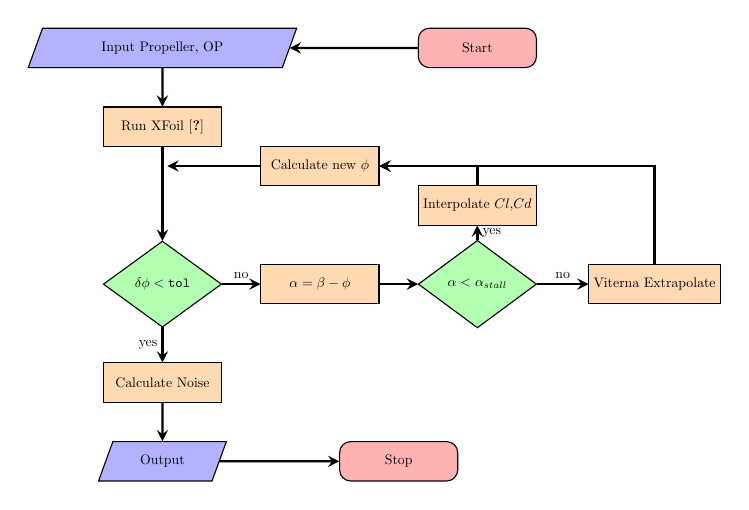
\begin{tikzpicture}[node distance=2cm, scale=0.5, transform shape]

\node (in1) [io] {Input Propeller, OP};
\node (start) [startstop, right of=in1, xshift=6cm] {Start};

\node (pro1) [process, below of=in1] {Run XFoil \cite{xfoil}};
\node (midin) [below of=pro1, yshift=1cm] {};
\node (pro5) [process, right of=midin, xshift=2cm] {Calculate new $\phi$};
\node (dec1) [decision, below of=pro1, yshift=-2cm] {$\delta \phi < \texttt{tol}$};
\draw [arrow] (pro1) -- (dec1); 

\node (pro2a) [process, below of=dec1, yshift=-0.5cm] {Calculate Noise};

\node (pro2b) [process, right of=dec1, xshift=2cm] {$\alpha = \beta - \phi$};
\node (dec2) [decision, right of=pro2b, xshift=2cm] {$\alpha < \alpha_{stall}$};
\node (pro3) [process, above of=dec2] {Interpolate $Cl$,$Cd$};
\node (pro4) [process, right of=dec2, xshift=2.5cm] {Viterna Extrapolate};

\draw [arrow] (pro2b) -- (dec2);

\draw [arrow] (dec2) -- node[anchor=south, right] {yes} (pro3);
\draw [arrow] (dec2) -- node[anchor=east, above] {no} (pro4);


\node (out1) [io, below of=pro2a] {Output};
\node (stop) [startstop, right of=out1, xshift = 4cm] {Stop};

\draw [arrow] (start) -- (in1);
\draw [arrow] (in1) -- (pro1);
\draw [arrow] (dec1) -- node[anchor=east] {yes} (pro2a);
\draw [arrow] (dec1) -- node[anchor=south] {no} (pro2b);
\draw [arrow] (pro3) |- (pro5);
\draw [arrow] (pro4) |- (pro5);
\draw [arrow] (pro5) -- (midin);
\draw [arrow] (pro2a) -- (out1);
\draw [arrow] (out1) -- (stop);

\end{tikzpicture}

\end{document}